\section{HH signatures}

Probing the HH self-coupling is extremely interesting, but in the SM, the dominant gluon-gluon-fusion (ggF) cross-section is fantastically low at $\sigma_{ggF\,HH}^{\text{SM}} = 31.05$.\footnote{This includes next-next-to-leading order (NNLO) corrections with an the infinite top limit. The uncertainties  of $\sigma_{ggF\,HH}^{\text{SM}} = 31.05$ $\pm 3\%$ (PDF+$\alpha_{s}$) $^{+ 6\%}_{-23\%}$ (Scale + $m_{\text{top}}$)\,fb~\cite{Grazzini_2018} for a Higgs mass of 125 \GeV.}.
\hl{Could I give a rule of thumb for how much smaller this is c.f. other processes at the LHC?}

There are two diagrams that contribute to this process at leading order, as shown in \Fig{\ref{fig:ggF_feyn_dias}}, where there are two diagrams, the box diagram (\Fig{\ref{fig:ggF_feyn_dias}}) where the top loop radiates two Higgs bosons, and a triangle diagram (\Fig{\ref{fig:ggF_feyn_dias}}) which is includes the coupling of interest since the Higgs radiated by the top produces another two Higgses by its self-coupling. 
%In the SM, we see HH events 2000x less often than single Higgs events 
Although the process is so rare that we won't see it until the HL-LHC \cite{hh-proj}, we could see it sooner if the Higgs self-coupling deviates from the expectation. In the $\kappa$ framework, we parametrize the deviations of the couplings from the SM values, i.e, $\kappa_\lambda = \lambda / \lambda_{SM}$, and we can parametrize the deviations of the SM couplings from the other values similarly as well.

\begin{figure}[h]
    \centering
    \subfloat[The box diagram.]{
        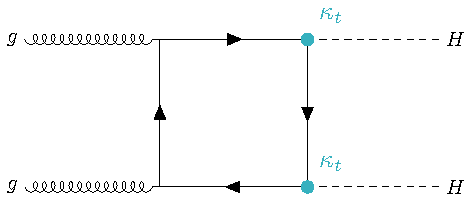
\includegraphics[width=0.45\textwidth]{\figpath/ggF_box.pdf}
        \label{fig:box}
    }
    \subfloat[The triangle diagram.]{
        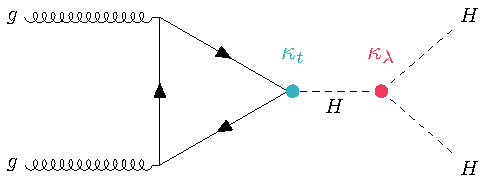
\includegraphics[width=0.45\textwidth]{\figpath/ggF_tri.pdf}
        \label{fig:triangle}
    }
    \caption{The leading order gluon-gluon fusion di-Higgs production Feynman diagrams.}
    \label{fig:ggF_feyn_dias}
\end{figure}

In \Fig{\ref{fig:box_tri}}, you can see the contribution from each of the terms individually, and the interference between the two processes.
In the SM, this process is suppressed to destructive interference between these two diagrams.

\begin{figure}[h]
    \centering
    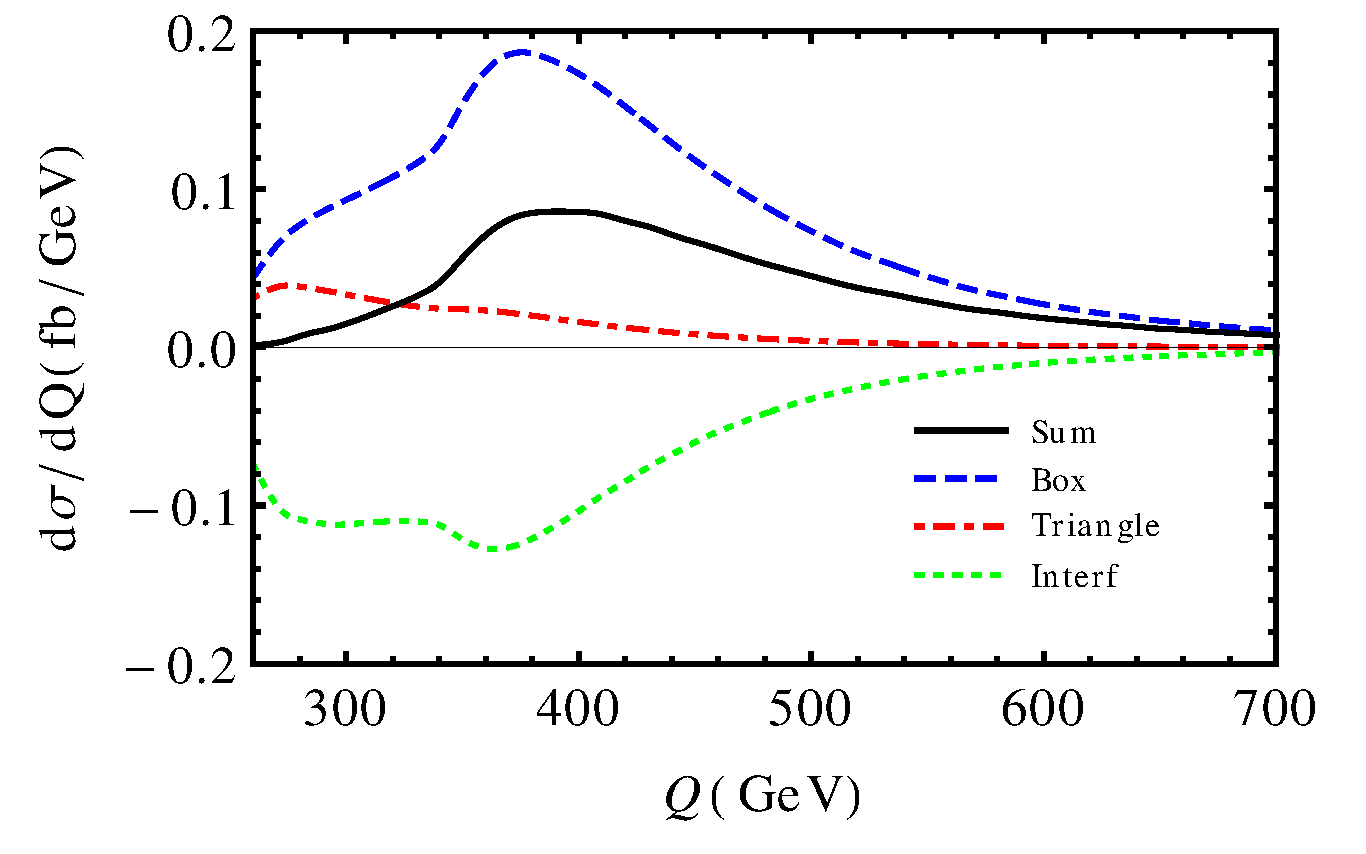
\includegraphics[width=0.8\textwidth]{figures/my_dihiggs/box_triangle_diagram.pdf}
    \caption{Impact of the interference of the box and triangle diagrams for ggF HH production.}
    \label{fig:box-tri}
\end{figure}

%%%%%%%%%%%%%%%%%%%%%%%%
%     VBF
%%%%%%%%%%%%%%%%%%%%%%%%

\textbf{from James - need to rephrase sentences}
The second-leading \HH production process is vector boson fusion (VBF), which has a SM cross-section over an order of magnitude smaller than ggF, at $\sigma_{VBF\,\HH}^{SM} = 1.726$ $\pm 2.1\%$ (PDF+$\alpha_{s}$) $^{+0.03\%}_{-0.04\%}$(Scale)\,fb~\cite{Dreyer_2018} at next-to-next-to-next-to-leading order (N3LO) for a SM Higgs boson with mass of 125 \GeV. 

\begin{figure}[t]
    \centering
    \subfloat[$\mathcal{M}_{\lambda}$]{
        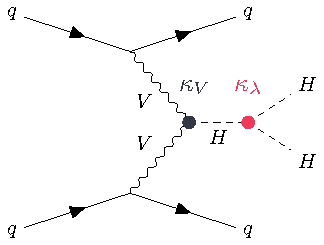
\includegraphics[width=0.33\textwidth]{\figpath/VBF_kvkl.pdf}
        \label{"fig:VBF_kvkl"}
    }
    \subfloat[$\mathcal{M}_{2V}$]{
        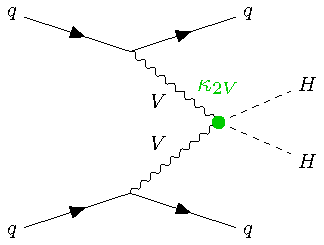
\includegraphics[width=0.33\textwidth]{\figpath/VBF_k2v.pdf}
        \label{"fig:VBF_k2v"}
    }
    \subfloat[$\mathcal{M}_{V}$]{
        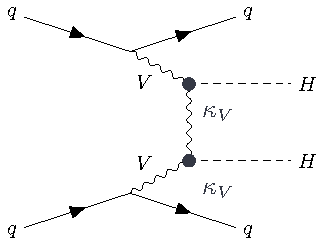
\includegraphics[width=0.33\textwidth]{\figpath/VBF_kvkv.pdf}
        \label{"fig:VBF_kvkv"}
    }
    \caption{The three tree-level vector boson fusion di-Higgs production Feynman diagrams. A convention the matrix elements names is given in the captions of the respective diagrams.}
    \label{fig:VBF_feyn_dias}
\end{figure}

\begin{figure}
    \centering
    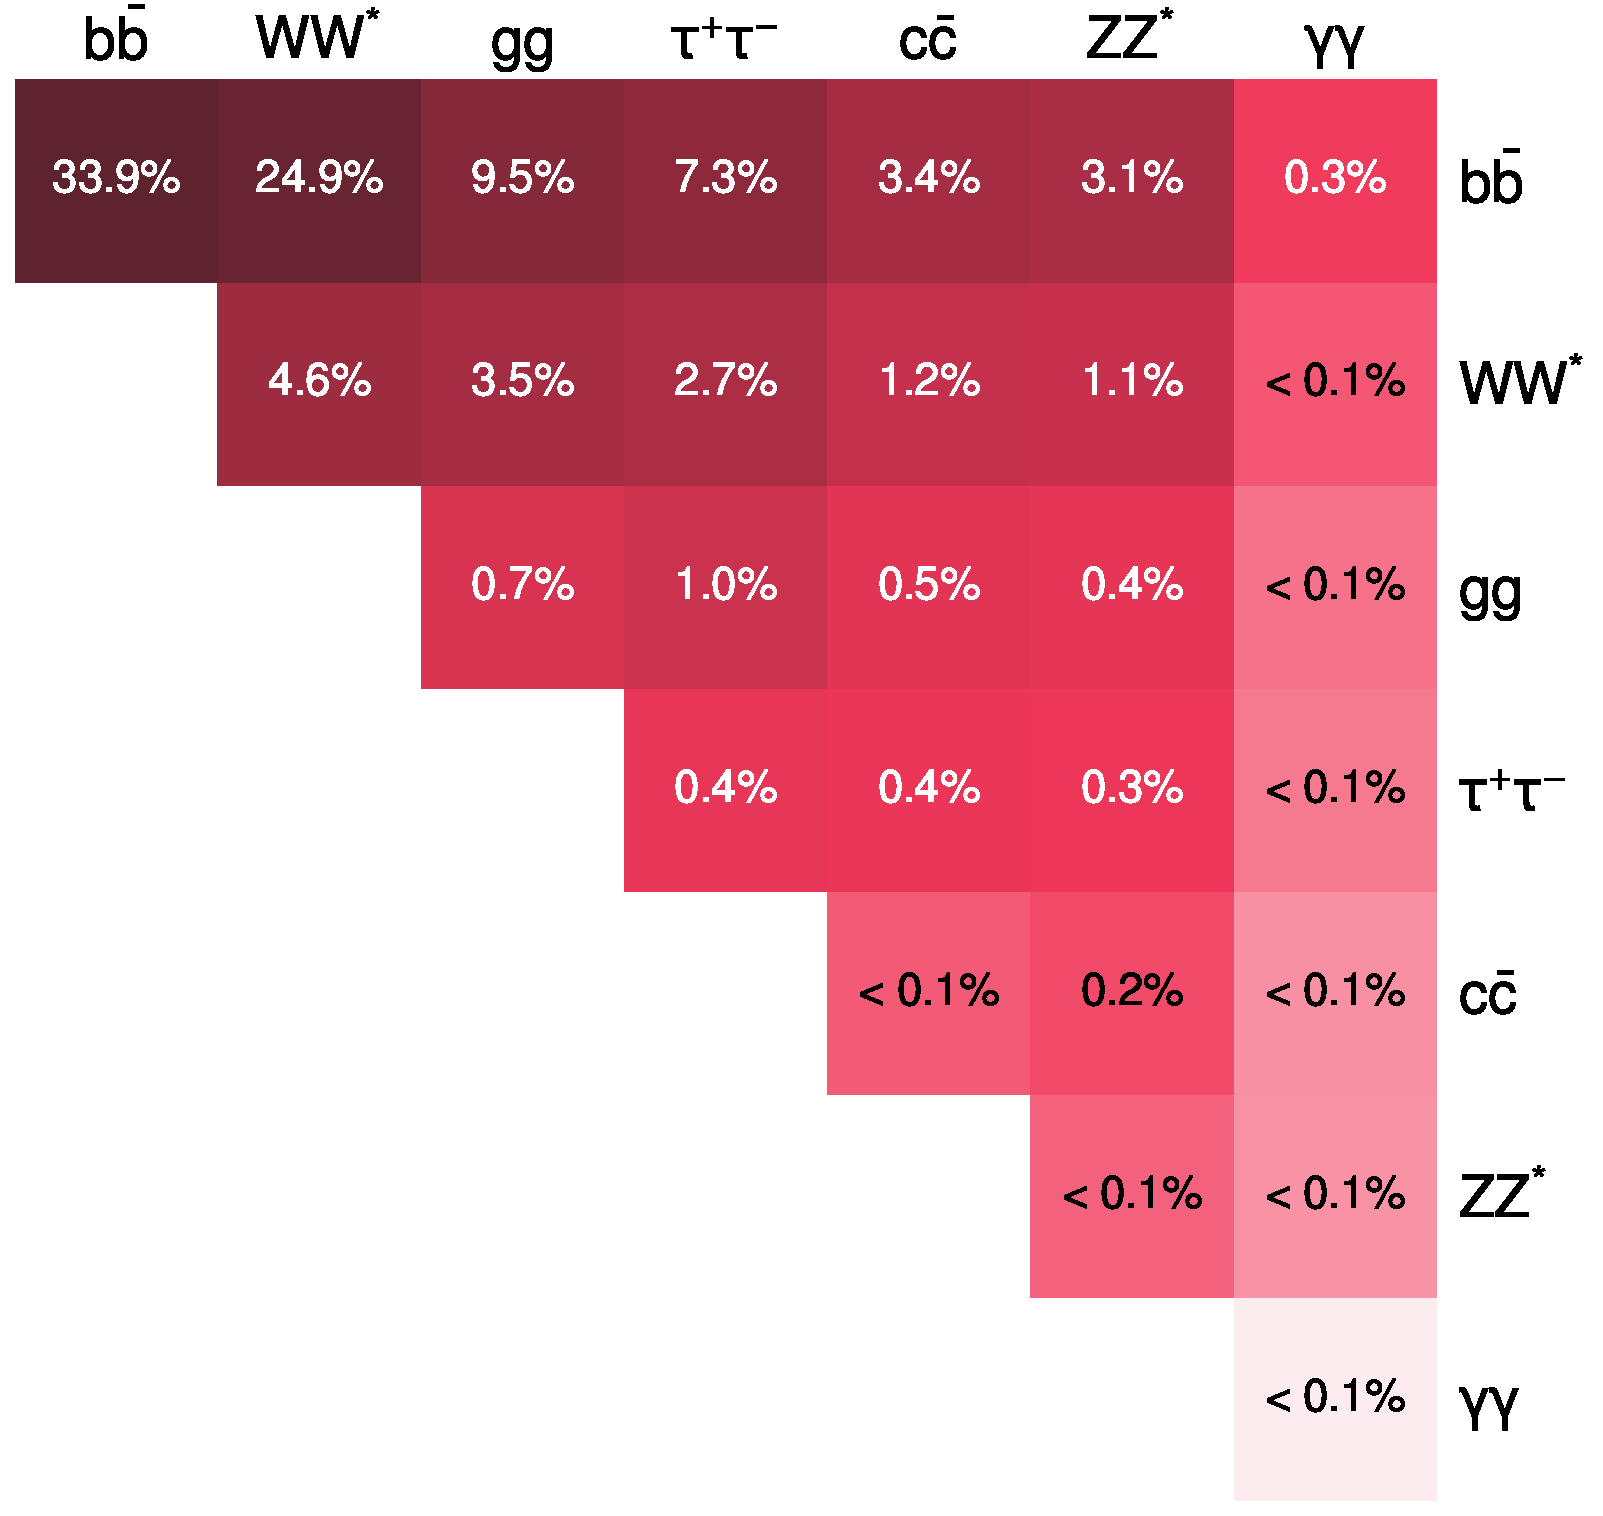
\includegraphics[width=0.7\textwidth]{\figpath/hhbr-dkpink}
    \caption{Branching ratios of the di-Higgs at the LHC.}
    \label{fig:branching-ratios}
\end{figure}

\begin{figure}
    \centering
    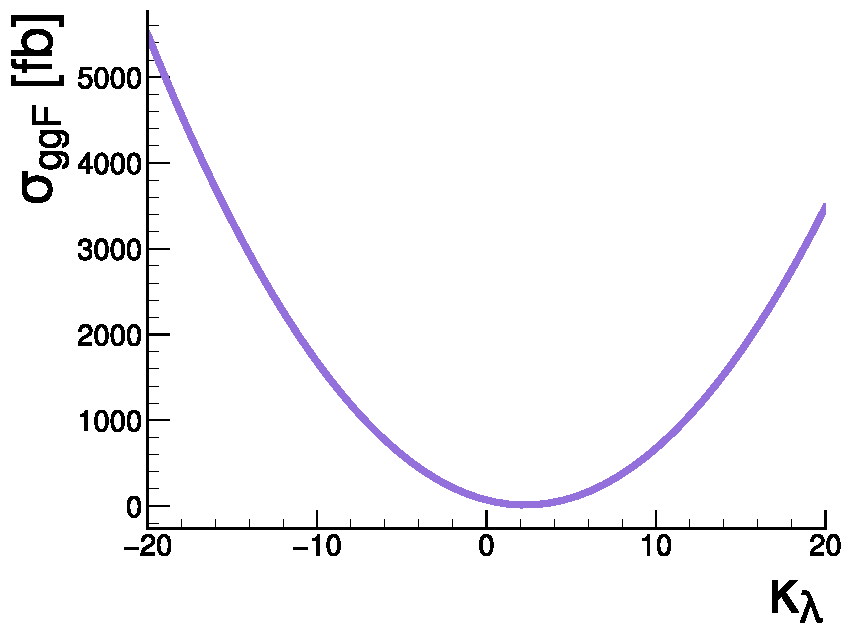
\includegraphics[width=0.5\textwidth]{figures/my_dihiggs/kl_ggF_theory_xsec.pdf}
    \caption{Cross-section dependence on \kl.}
    \label{fig:truth-hh-presel}
\end{figure}

\begin{figure}
    \centering
    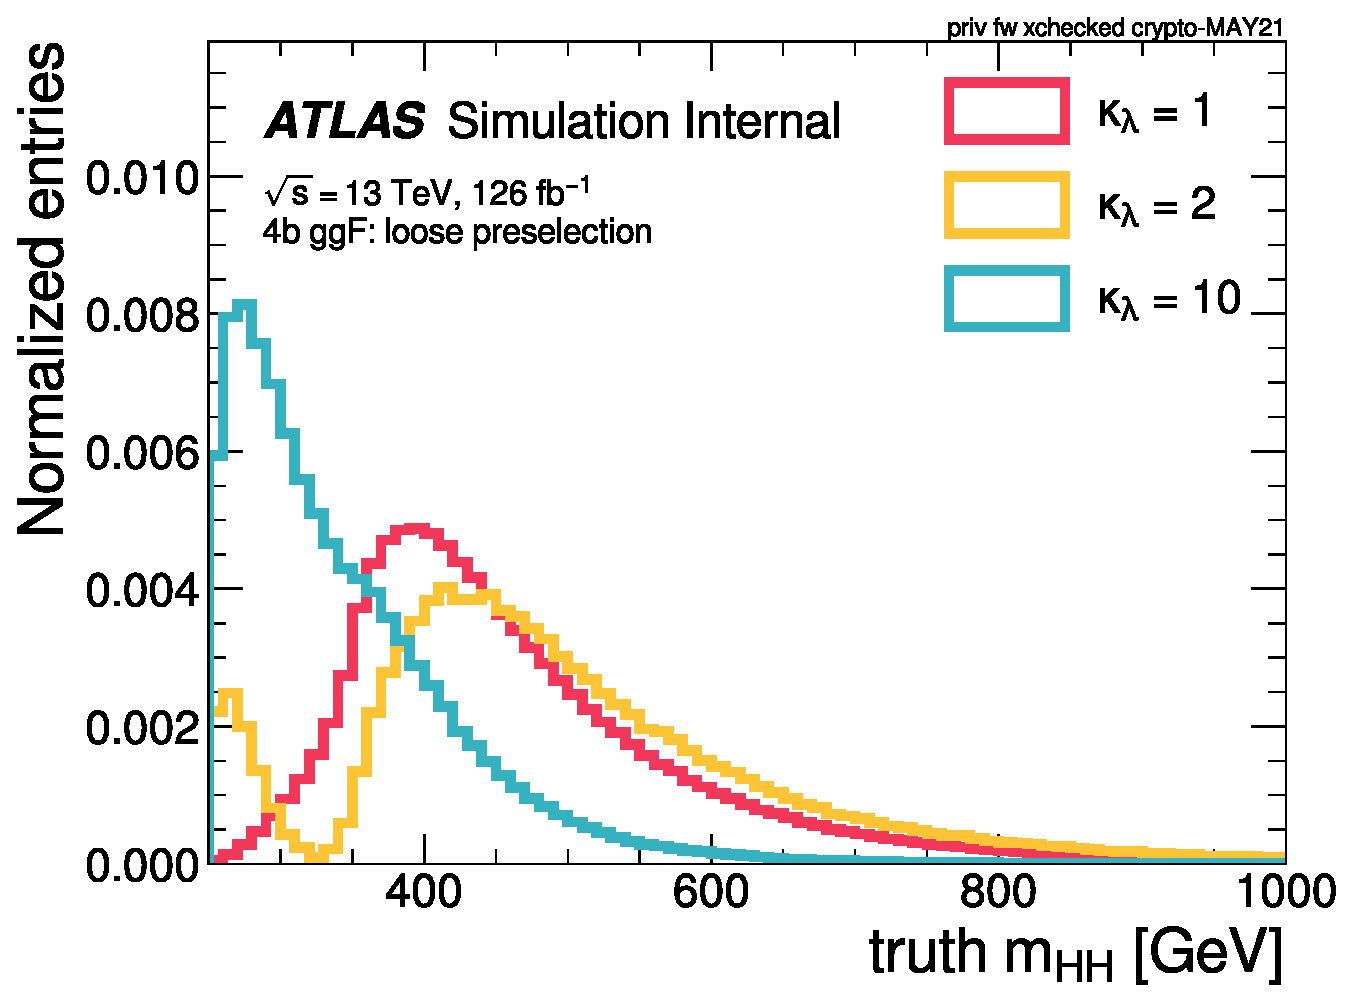
\includegraphics[width=0.7\textwidth]{figures/my_dihiggs/truth_mhh_ggf_common_presel.pdf}
    \caption{Impact of the destructive interference for the \kl variations.}
    \label{fig:truth-hh-presel}
\end{figure}